% ----------------------------------------------------------------------------------------\
% ---------------------------------------------------------------------------------------\
% --------------------------------------------------------------------------------------\
\section{Investigación}
% ----------------------------------------------------------------------------------------\
% ---------------------------------------------------------------------------------------\
% --------------------------------------------------------------------------------------\

% ----------------------------------------------------------------------------------------\
% ---------------------------------------------------------------------------------------\
\subsection{Fundamentos de redes bayesianas}
% ----------------------------------------------------------------------------------------\
% ---------------------------------------------------------------------------------------\


% ----------------------------------------------------------------------------------------\
% Investiga y redacta un breve resumen (máximo una cuartilla) sobre
%  qué son las redes bayesianas y para qué se utilizan.
\subsection*{Redes bayesianas}
% ----------------------------------------------------------------------------------------\
Las redes bayesianas nos permiten modelar un sistema mediante un conjunto de variables y sus respectivas relaciones de dependencia, permitiendo llevarlo a inferencia bayesiana con la que podemos estimar la probabilidad de relacionarse con variables no conocidas, con base a las conocidas. Las redes bayesianas generalmente también incluirán un conjunto de tablas de probabilidad, indicando las probabilidades para los valores verdadero o falso de las variables. 
El punto principal de las Redes Bayesianas es permitir que se realice una inferencia probabilística. Esto significa que la probabilidad de cada valor de un nodo en la red bayesiana se puede calcular cuando se conocen los valores de las otras variables.

\\ 

Una red Bayesiana consta de:
\begin{itemize} 
    \item \textbf{Cualitativa} que describe las relaciones entre las distintas variables
    \item \textbf{Cuantitativa} que describe la fuerza de dichas relaciones mediante probabilidades condicionadas
\end{itemize}

\\

Estos modelos tienen amplios usos en la clasificación, predicción, diagnostico, que brindan información sobre como se relaciones las variables llevándolos a un enfoque de causa y efecto, donde los vértices de la gráfica representan variables llamados nodos. Los nodos se representan como círculos que contienen el nombre de la variable. Las conexiones entre los nodos se nombran aristas.
\\

Las redes Bayesianas se utilizan en una amplia gama de aplicaciones. Por ejemplo:

\begin{itemize}
    \item  En medicina, Las redes Bayesianas pueden ayudar a los médicos a evaluar la probabilidad de que un paciente tenga cierta enfermedad en función de los síntomas observados y los factores de riesgo.
    \item En finanzas, pueden utilizarse para evaluar riesgos y rendimientos en carteras de inversión.
    \item En reconocimiento de patrones, pueden utilizarse para clasificar imágenes o datos sensoriales.

    \item Predicción del tiempo: Pueden utilizarse para modelar la probabilidad de diferentes condiciones climáticas en función de variables como la temperatura, la presión atmosférica y la humedad.

\end{itemize}
En cada una de estas aplicaciones, las redes Bayesianas permiten modelar la incertidumbre y realizar inferencias probabilísticas sobre las variables de interés.

% ----------------------------------------------------------------------------------------\
% Explica la diferencia entre probabilidad condicional e independencia condicional, 
%  incliyendo ejemplos claros de cada uno.
\subsection*{Probabilidad condicional e independencia condicional}
% ----------------------------------------------------------------------------------------\

\begin{enumerate}
    \item Probabilidad Condicional:

La probabilidad condicional se refiere a la probabilidad de que ocurra un evento dado que otro evento ya ha ocurrido. Se denota como \( P(A | B) \), que es la probabilidad de que el evento \( A \) ocurra dado que el evento \( B \) ha ocurrido. La fórmula para calcular la probabilidad condicional es:

\[ P(A | B) = \frac{P(A \cap B)}{P(B)} \]

Lo que significa que la probabilidad de \( A \) dado \( B \) es igual a la probabilidad de que ocurran ambos \( A \) y \( B \) dividida por la probabilidad de que ocurra \( B \).

Un ejemplo es: supongamos que tenemos dos eventos \( A \) y \( B \), donde \( A \) representa sacar una carta roja de una baraja estándar de 52 cartas, y \( B \) representa sacar una carta de corazones. La probabilidad de sacar una carta roja dado que hemos sacado una carta de corazones se puede calcular utilizando la fórmula de probabilidad condicional:

\[ P(A | B) = \frac{P(A \cap B)}{P(B)} \]

Donde \( P(A \cap B) \) es la probabilidad de sacar una carta roja que también sea un corazón, y \( P(B) \) es la probabilidad de sacar una carta de corazones. Si la carta roja que hemos sacado también es un corazón, entonces la probabilidad de \( A \) dado \( B \) sería \( 1/13 \), ya que hay 13 cartas de corazones en total en una baraja de 52 cartas.

\item Independencia Condicional:

Es la situación en la que dos eventos son independientes dado un tercer evento. Formalmente, dos eventos \( A \) y \( B \) son independientes condicionalmente a un evento \( C \) si la probabilidad de \( A \) dado \( B \) no cambia incluso si sabemos que \( C \) ha ocurrido. Se denota como \( A \perp\!\!\!\perp B \,|\, C \).

Por ejemplo, consideremos tres eventos \( A \), \( B \) y \( C \), donde \( A \) representa sacar una carta roja de una baraja de cartas, \( B \) representa sacar una carta de corazones y \( C \) representa sacar una carta alta (as, rey, reina o jota). Si los eventos \( A \) y \( B \) son independientes condicionalmente a \( C \), esto significa que la probabilidad de sacar una carta roja que también sea un corazón no cambia incluso si sabemos que hemos sacado una carta alta. En este caso, si \( A \) y \( B \) son independientes condicionalmente a \( C \), entonces la probabilidad de \( A \) dado \( B \) sigue siendo \( 1/13 \), incluso después de que hemos sacado una carta alta.

% ----------------------------------------------------------------------------------------\
% Describe cómo se representa matemáticamente una red bayesiana y
%  el significado de los nodos y aristas en cada representación.
\subsection*{Representación Matematica}
% ----------------------------------------------------------------------------------------\
Una red Bayesiana se define como un par \( (G, \Theta) \), donde \( G \) es un grafo dirigido acíclico (DAG) y \( \Theta \) es un conjunto de tablas de probabilidad condicional (TPC). 

El grafo \( G \) consiste en un conjunto de nodos \( V \) y un conjunto de arcos \( E \). Cada nodo representa una variable aleatoria y cada arco representa una dependencia probabilística entre las variables. Las tablas de probabilidad condicional \( \Theta \) especifican la probabilidad de cada valor posible de cada variable condicionado a los valores de sus nodos padres.

Para representar la probabilidad conjunta de todas las variables en la red, utilizamos la regla del producto:

\[
P(\text{{variables}}) = \prod_{i=1}^{n} P(X_i \,|\, \text{{padres}}(X_i))
\]

donde \( X_i \) es la variable \( i \)-ésima en la red y \( \text{{padres}}(X_i) \) son los nodos padres de \( X_i \) en el grafo.

Por ejemplo, supongamos que tenemos dos variables \( A \) y \( B \) en una red Bayesiana, donde \( B \) depende de \( A \). Podemos representar esto como:

\[
P(A, B) = P(A) \cdot P(B \,|\, A)
\]

Aquí, \( P(A) \) es la probabilidad marginal de \( A \) y \( P(B \,|\, A) \) es la probabilidad condicional de \( B \) dado \( A \). La probabilidad conjunta de \( A \) y \( B \) se calcula multiplicando la probabilidad de \( A \) por la probabilidad condicional de \( B \) dado \( A \).

Ejemplo de una red Bayesiana y los significados de los nodos y aristas:

\begin{figure}[H]
    \centering
    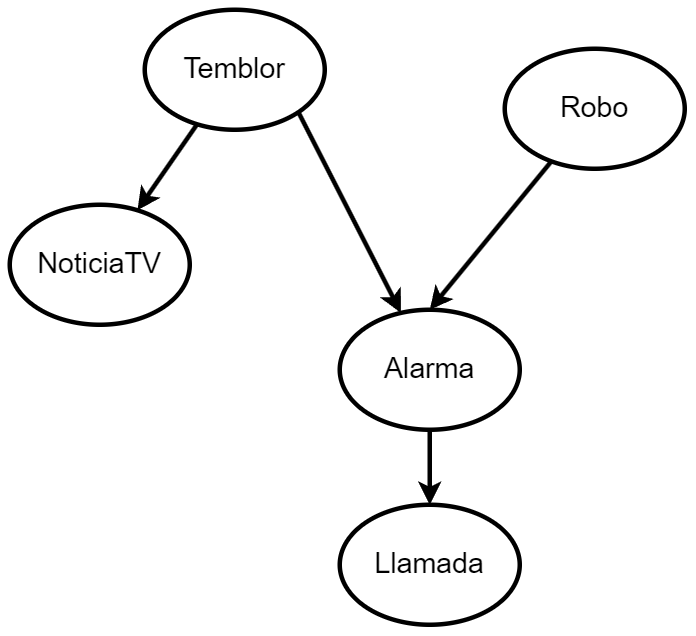
\includegraphics[width=0.35\linewidth]{IMA/RedesBayes.png} 
    \caption{Diagrama de una red Bayesiana} 
\end{figure}

Observemos estos elementos en la red Bayesiana:

\begin{itemize}
    \item Si hay un robo es más probable
    suene la alarma, lo que hace más probable que que reciba una llamada.
    
    \item Si recibo una llamada se incrementa
    la probabilidad de que haya sonado la alarma y por tanto de que me
    hayan robado
    
    \item Si oigo en la radio que ha habido un
    terremoto es más probable que éste haya ocurrido, lo que hace más
    probable que que suene la alarma.
    
    \item Si suena la alarma se incrementa la
    probabilidad de que haya ocurrido un terremoto y por tanto de que
    oiga la noticia en la television.
    
    \item Si suena la alarma y ocurre una de
    las causas (terremoto) , me creo menos que haya ocurrido el otro evento causante (robo)	
    
    \item Y viseversa, Sí suena la alarma y ocurre una de
    las causas (robo) me creo menos que haya ocurrido el otro evento causante (terremoto)
\end{itemize}

Notemos como los nodos y aristas en la red Bayesiana representan las relaciones probabilísticas entre las variables y cómo se propagan las probabilidades a través de la red. Siendo una herramienta poderosa para modelar sistemas complejos y realizar inferencias probabilísticas.
Dependiendo de nuestro enfoque de estudio, podemos utilizar las redes bayesianas para modelar sistemas complejos y realizar inferencias probabilísticas.

Elementos de una red Bayesiana:
\begin{itemize} 
    \item Nodos: Cada nodo en el grafo representa una variable aleatoria. Que representan aspectos del sistema que estamos modelando.
    \item Aristas: Las aristas representan las relaciones entre las variables. Una arista que va desde el nodo A al nodo B indica que el nodo B es dependiente del nodo A. Esto puede interpretarse como "el nodo A causa o influye en el nodo B".
\end{itemize}

Distribuciones de probabilidad condicional

\begin{itemize}
    \item Para cada nodo en la red, este tiene asociada una distribución de probabilidad condicional que describe la probabilidad de los posibles valores del nodo dado los valores de sus nodos padres.
    \item Las Distribuciones de probabilidad condicional reflejan las relaciones causales entre las variables representadas por los nodos. Por ejemplo, en una red que modela el clima y la probabilidad de lluvia, la Distribuciones de probabilidad condicional del nodo "lluvia" podría depender de los nodos "humedad"\ y "neblina".
\end{itemize}

Ventajas y limitaciones de las redes bayesianas

Las ventajas de las Redes Bayesianas son las siguientes:

\begin{enumerate} 
    \item Las Redes Bayesianas representan visualmente todas las relaciones entre las variables en el sistema con arcos de conexión.
    \item Es fácil reconocer la dependencia e independencia entre varios nodos.
    \item Las redes bayesianas pueden manejar situaciones en las que el conjunto de datos está incompleto ya que el modelo da cuenta de las dependencias entre todas las variables.
    \item Las redes bayesianas pueden mapear escenarios donde no es factible/práctico medir todas las variables debido a las limitaciones del sistema (costos, falta de suficientes sensores, etc.)
    \item Ayuda a modelar sistemas ruidosos.
    \item Se puede utilizar para cualquier modelo de sistema, desde todos los parámetros conocidos hasta ningún parámetro conocido.
\end{enumerate}

Las limitaciones de las Redes Bayesianas son las siguientes:

\begin{enumerate} 
    \item Todas diferentes caminos o ramificaciones que pueden tomar los nodos en el grafo, deben ser calculadas para calcular la probabilidad de cualquier rama.
    \item La calidad de los resultados de la red depende de la calidad de las creencias o modelos previos. Una variable es solo una parte de una red bayesiana si crees que el sistema depende de ella.
    \item El cálculo de la red es NP-duro, por lo que es muy difícil y posiblemente costoso.
    \item Los cálculos y probabilidades utilizando la regla y marginación de Bayes pueden volverse complejos.
\end{enumerate}